\documentclass{article}
\usepackage{graphicx}
\usepackage{float}
\usepackage{epstopdf}

\begin{document} 
\begin{center}
{\bf \Large  Homework 5} \\
\end{center}
Chien-Pin Chen\\
05/13/2016

\begin{figure}[h]
\begin{center}
\includegraphics[width=0.6\textwidth]{fig1.jpg}
\end{center}
\end{figure}

\noindent The figure shows a robot moving left with the average velocity of $0.8cm/s$.
While moving, it measures each second ($\Delta T = 1s$) the distance from the obstacle
behind it (the corner) and the obstacle in front of it (the wall). In this scenario,
we consider the corner as the reference point, i.e., with the coordinate 0. 
In order to simultaneously estimate the robot position, as well
as the position of the wall, we use the state vector $\underline{x}$ with three components: 
$x_1$ is the robot position measured from the corner, $x_2$ is the robot velocity with
positive direction towards the wall and $x_3$ is the wall position measured from
the corner.  $y_1$ is the measurement of the distance from the robot to the corner
and $y_2$ is the measurement of the distance from the robot to the wall. A linear model describing this scenario is
\begin{equation}
  \underline{x}(k+1)=\left[ 
  \begin{array}{ccc}
     1 & 1 & 0  \\
     0 & 0 & 0  \\
     0 & 0 & 1 
  \end{array}
   \right] \underline{x}(k)+
   \left[ 
  \begin{array}{c}
     0   \\
     0.8   \\
     0
  \end{array}
   \right]+ \left[
     \begin{array}{c}
     0   \\
     0.1   \\
     0
  \end{array}
   \right] w(k)
\end{equation}
where the Gaussian random variable $w(k)$ has zero mean and variance 1. 
The observation model is
\begin{equation}
 \underline{y}(k) =\left[
     \begin{array}{ccc}
     1 & 0 &  0  \\
     -1 & 0 & 1   
  \end{array}
   \right] \underline{x}(k)+\underline{\theta}(k)
\end{equation}
where the covariance matrix of Gaussian measurement noise $\underline{\theta}$ is $diag(10, 10)$. All variables in the above equations are expressed in $cm$ and $cm/s$. The course webpage provides you the sequence of the measurements $y_1$ and $y_2$ recorded for 
$k = 1, 2,... $ in the file {\bf roboMes.mat}. The data are organized in such a way that $y(1, k)$ denotes the measurement $y_1(k)$ and $y(2, k)$ denotes the measurement $y_2(k)$, where $k=1,2,3...$

Design the Kalman filter that takes the measurement sequences and produces the estimation sequences of the robot position, its velocity and the distance between the wall and the corner.
\begin{itemize}
\item[a)] Plot the measurements on the same diagram. 
\item[b)] Plot the estimated robot position and the corresponding variance. 
\item[c)] Plot the estimated wall position and the corresponding variance. 
\end{itemize}
What is the precision in estimating the position of the robot and the wall ?
Compare the precision to the intensity of measurement errors. Comment your
results and trends in data.\\
\textbf{ANS:}\\
In Kalman filter, equation 1 can refer to the equation in prediction step:
\begin{equation}
	\underline{x}_{k + 1}  = \Phi \underline{x}_k  + \Lambda u_k  + \Gamma w_k 
\end{equation}
then, for computing, I could set :
\begin{equation}
	\Phi  = \left[ {\begin{array}{*{20}c}
	   1 & 1 & 0  \\
	   0 & 0 & 0  \\
	   0 & 0 & 1  \\
	\end{array}} \right]{\rm{, }}\Lambda  = \left[ {\begin{array}{*{20}c}
	   0  \\
	   {0.8}  \\
	   0  \\
	\end{array}} \right],{\rm{ }}\Gamma  = \left[ {\begin{array}{*{20}c}
	   0  \\
	   {0.1}  \\
	   0  \\
	\end{array}} \right],{\rm{ and }}Q = {\mathop{\rm var}} (w(k)) = 1
\end{equation}

\noindent And, equation 2 can refer to the equation in observation step:
\begin{equation}
	\underline{y}_k  = {\rm H}\underline{x}_k  + Du_k  + \underline{v}_k 
\end{equation}
then, for computing, I could set :
\begin{equation}
	{\rm H} = \left[ {\begin{array}{*{20}c}
	   {\begin{array}{*{20}c}
	   1 & 0 & 0  \\
	\end{array}}  \\
	   {\begin{array}{*{20}c}
	   { - 1} & 0 & 1  \\
	\end{array}}  \\
	\end{array}} \right],{\rm{ and }}R = {\mathop{\rm var}} (\theta (k)) = \left[ {\begin{array}{*{20}c}
	   {10} & 0  \\
	   0 & {10}  \\
	\end{array}} \right]
\end{equation}
\textbf{When using Kalman Filter:}\\
Using following equations for prediction step:
\begin{eqnarray}
	\begin{array}{l}
	 \hat{ \underline{x}}_{k + 1}  = \Phi  \hat{ \underline{x}}_k  + \Lambda u_k  \\ 
	 \underline{P}_{k + 1}  = \Phi \underline{P}_k \Phi ^T  + \Gamma Q\Gamma ^T  \\ 
	 \end{array}
\end{eqnarray}
Next, use following equation for observation step:
\begin{equation}
	\underline{y}_k  = {\rm H}x_k  + \theta _k 
\end{equation}
but, in this homework, I could the data in \textbf{roboMes.mat} as the result of $\underline{y}_k$\\
In update step, I use following equation:
\begin{equation}
	\hat{\underline{x}}_k ( + ) = \hat{\underline{x}}_k ( - ) + K(\underline{y} - \hat{\underline{x}}_k ( - ))
\end{equation}
and, using following equations for computing $K$ and $P(+)$:
\begin{eqnarray}
	\begin{array}{l}
	 K = P( - ){\rm H}^T ({\rm H}P( - ){\rm H}^T  + R)^{ - 1}  \\ 
	 P( + ) = ({\rm I} - K{\rm H})P( - ) \\ 
	 \end{array}
\end{eqnarray}
Before using those equation in MATLAB to design kalman filter, I still need to set initial guess for $\hat{\underline{x}}_0$ and $\underline{P}_0$.\\
\textbf{For $\hat{\underline{x}}_0$}, I use the first element of the measurement ($y$) to set initial guess of $\hat{\underline{x}}_0 (1)$ and $\hat{\underline{x}}_0 (3)$, 
and I use average velocity ($0.8 cm/s$) as initial guess of $\hat{\underline{x}}_0 (2)$. Therefore, the initial guess of $\hat{\underline{x}}_0$:
\begin{equation}
\hat{\underline{x}}_0  = \left[ {\begin{array}{*{20}c}
   {E\{ y_1 (1)\} }  \\
   {E\{ x_2 (0)\} }  \\
   {E\{ y_1 (1) + y_2 (1)\} }  \\
\end{array}} \right] = \left[ {\begin{array}{*{20}c}
   {\hat{\underline{y}}_1 (1)}  \\
   {0.8}  \\
   {\hat{\underline{y}}_1 (1) + \hat{\underline{y}}_2 (1)}  \\
\end{array}} \right]
\end{equation}
\textbf{For initial guess of $P_0$}, I could set each element refer to what I guess for $\hat{\underline{x}}_0$.\\
$P_{11}$ is the variance of the position of robot ($\hat{\underline{x}}_1 (0)$), I could set as:
\begin{equation}
	P_{11}  = {\mathop{\rm var}} (x_1 (0)) = {\mathop{\rm var}} (y_1 (1)) = \sigma _\theta ^2 
\end{equation}
$P_{33}$ is the variance of the position of wall ($\hat{\underline{x}}_3 (0)$), I could set as:
\begin{equation}
	P_{33}  = {\mathop{\rm var}} (x_3 (0)) = {\mathop{\rm var}} (y_1 (1) + y_2 (1)) = {\mathop{\rm var}} (2*\theta (k)) = 2\sigma _\theta ^2 
\end{equation}
$P_{12}$ and $P_{21}$ are the covariance of $\hat{\underline{x}}_0 (1)$ and $\hat{\underline{x}}_0 (2)$, which are independent to each other.
$P_{23}$ and $P_{32}$ are the covariance of $\hat{\underline{x}}_0 (3)$ and $\hat{\underline{x}}_0 (2)$, which are also independent to each other.
Therefore, I could set as:
\begin{equation}
	P_{12}  = P_{21}  = P_{23}  = P_{32}  = 0
\end{equation}
$P_{13}$ and $P_{31}$ are the covariance of $\hat{\underline{x}}_0 (1)$ and $\hat{\underline{x}}_0 (3)$, and I could compute as:
\begin{eqnarray}
	\begin{array}{l}
		P_{13}  = P_{31}  = {\mathop{\rm cov}} (x_3 (0),x_1 (0)) = E\{ (\hat x_3 (0) - x_3 (0))(\hat x_1 (0) - x_1 (0))\}  \\ 
	 	P_{13}  = E\{ (y_1 (1) + y_2 (1) - x_3 (0))(y_1 (1) - x_1 (0))\}  \\ 
	 	P_{13}  = E\{ (\theta _{y1}  + \theta _{y2} )(\theta _{y1} )\}  = E\{ \theta _{y1}^2 \}  + E\{ \underbrace {\theta _{y1} \theta _{y2} }_0\}  = \sigma _\theta ^2  \\ 
	 \end{array}
\end{eqnarray}
$P_{22}$ is the variance of the robot velocity ($\underline{x}_2$), I could set as:
\begin{equation}
	P_{22}  = {\mathop{\rm var}} \{ x_2 \}  = {\mathop{\rm var}} \{ \Gamma w_2 (k)\}  = \Gamma _2^2  = (0.1)^2 
\end{equation}
Now, the initial guess of $P_0$ could set as:
\begin{equation}
P_0  = \left[ {\begin{array}{*{20}c}
   {\sigma _\theta ^2 } & 0 & {\sigma _\theta ^2 }  \\
   0 & {(0.1)^2 } & 0  \\
   {\sigma _\theta ^2 } & 0 & {2\sigma _\theta ^2 }  \\
\end{array}} \right]
\end{equation}
Finally, I could use above equations in MATLAB to use kalman filter to produce the estimation of the robot position, its velocity, and the distance between the wall and the corner.\\
\textbf{a)} After loading \textbf{roboMes.mat}, I can plot the measurements as:
\begin{figure}[H]
\begin{center}
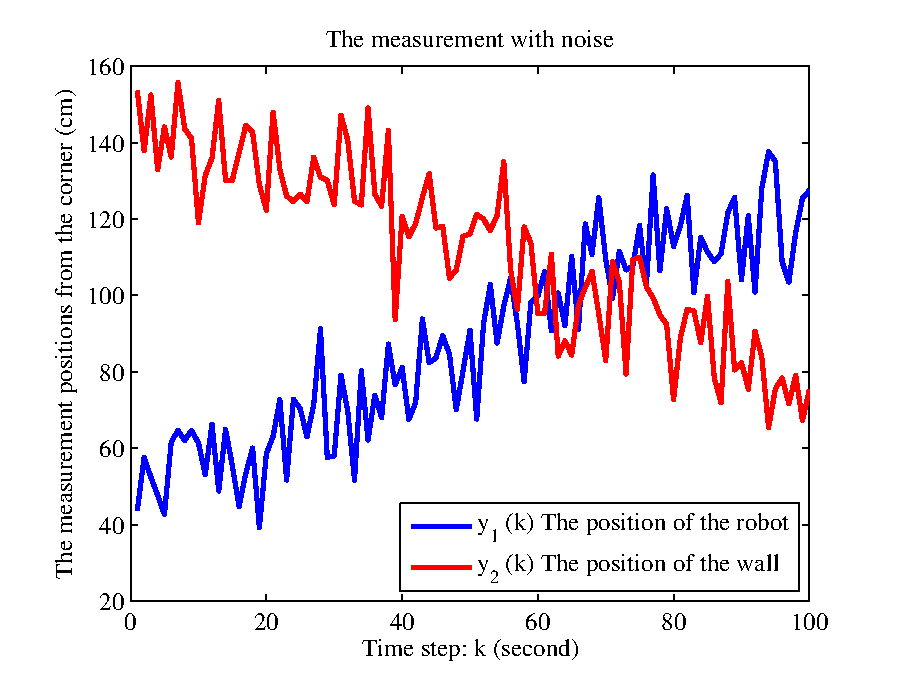
\includegraphics[scale=0.6]{hw5_y12.eps}
\caption{The measurement with noise.}
\end{center}
\end{figure}
\noindent \textbf{b) and c)}\\  
after using kalman filter, I get the estimation of the position of the robot and the wall:
\begin{figure}[H]
\begin{center}
\includegraphics[scale=0.6]{hw5_estX13.eps}
\caption{The expectation of the position of the robot and the wall.}
\end{center}
\end{figure}
And, the variance of the position of the robot and the wall:
\begin{figure}[H]
\begin{center}
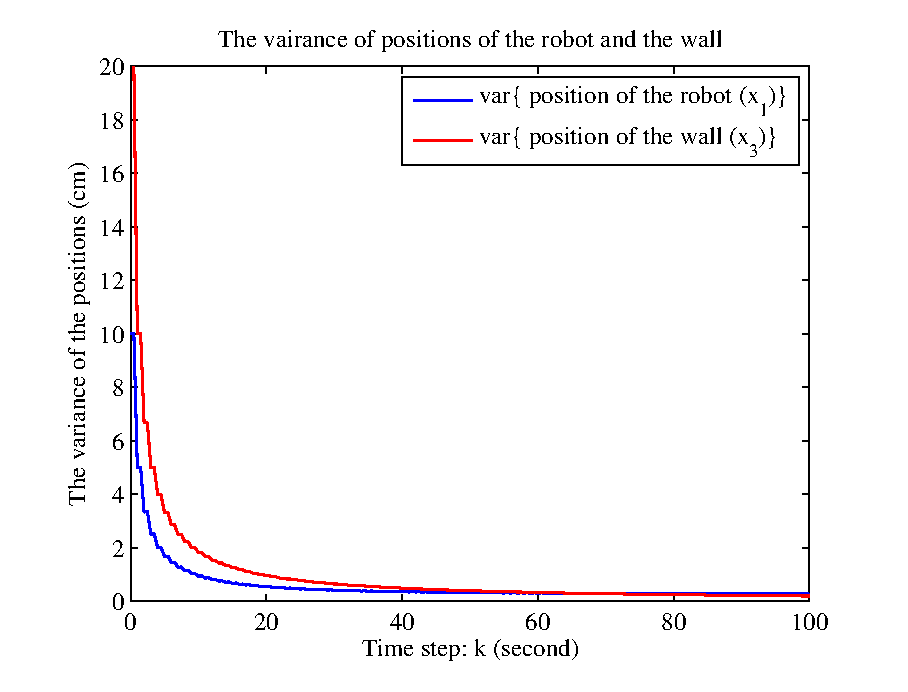
\includegraphics[scale=0.7]{hw5_varX13.eps}
\caption{The variance of the position of the robot and the wall.}
\end{center}
\end{figure}
\noindent The precision in estimating the position of the robot and the wall are the variance of the robot and the wall, so I refer to figure 3 to find 
the result and the trends of precision.After using kalman filter, the precision of the position of the robot is decreased from 10 to 0.2682, and 
the precision of the position of the wall is decreased from 20 to 0.198. The intensity of measurement  errors are constant ($var(\theta)=diag(10,10)$), 
while the precision of the position of the robot and the wall will decrease after each measuring update. 
 
\end{document}

